\addcontentsline{toc}{section}{Combined Pulley (1)}
\section*{Combined Pulley}

\subsection*{Problem}
\begin{wrapfigure}{r}{\textwidth / 2}
    \centering
    \vspace{-.75cm}
    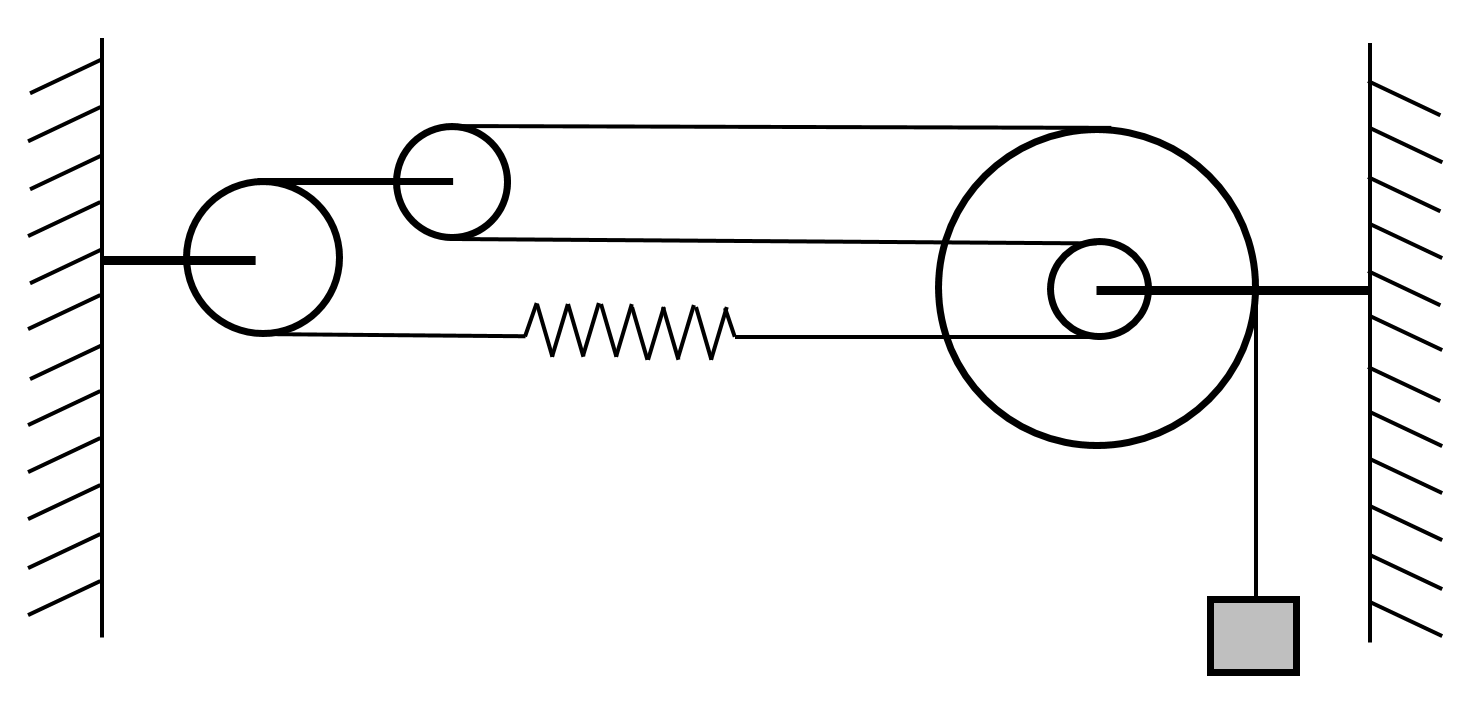
\includegraphics[width = \textwidth / 2]{P-1}
    \caption{}
    \labelf{P-1}
    \vspace{-4cm}
\end{wrapfigure}

How much will the weight $m$ shown on \reff{P-1} descend
after hanging it on the rope?
The coaxial pulleys are attached to each other
and the ratio of their radii is $n > 1$.
The stiffness of the spring is $k$.
There is no sliding.

\vspace{2cm}

\subsection*{Solution}

\begin{wrapfigure}{r}{.6\textwidth}
    \centering
    \vspace{-.75cm}
    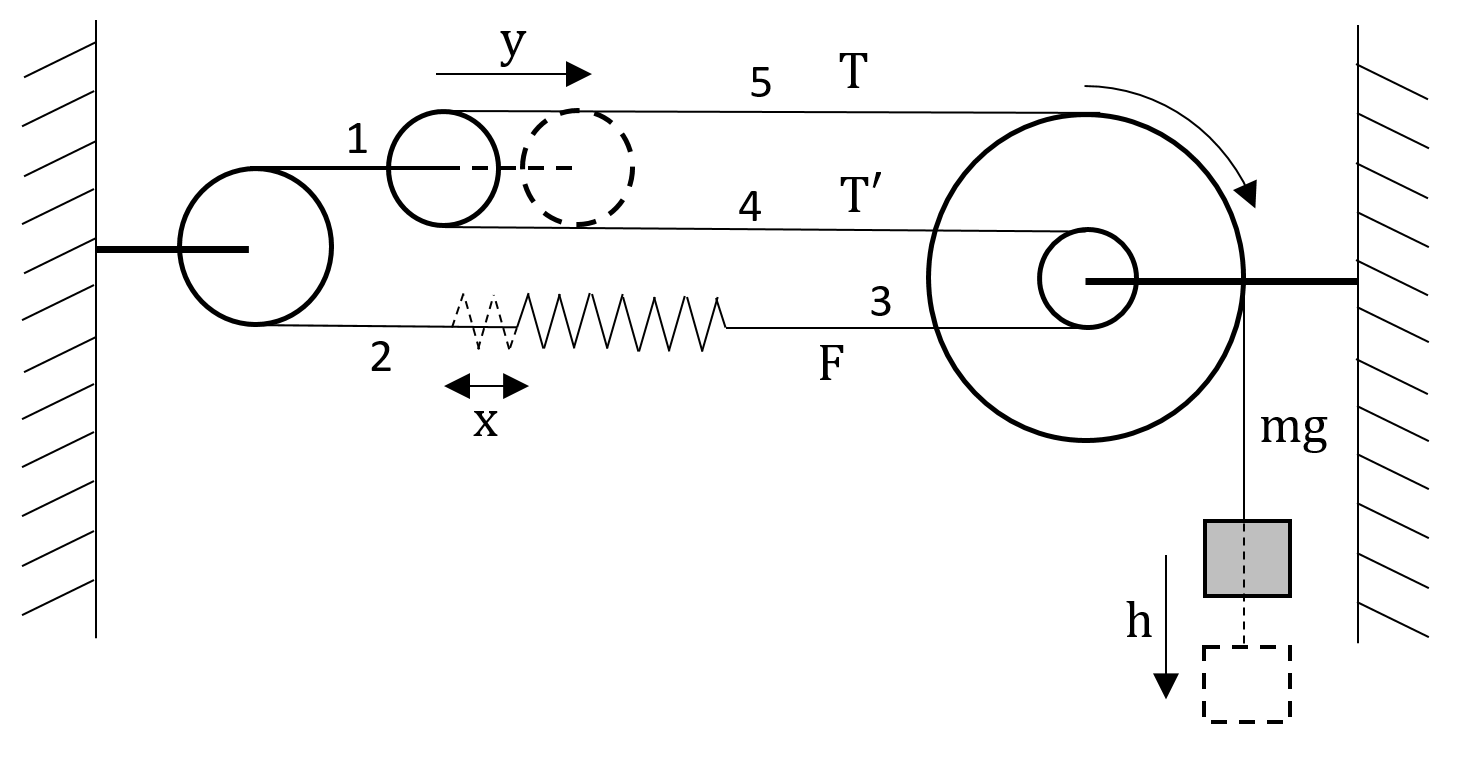
\includegraphics[width = .6\textwidth]{S-1}
    \caption{The initial (solid lines) and the final (dashed lines)
        states of the system.}
    \labelf{S-1}
    \vspace{-1.5cm}
\end{wrapfigure}

For the final state \reff{S-1} we have the following equilibrium conditions
\begin{equation}
\begin{split}
    T &= T' \\
    F &= T + T' \\
    F + nmg &= T' + nT
\end{split}
\end{equation}
from where the value of $F$, and consequently
the spring deformation $x$ can be found.
\begin{equation}
    x = \frac{F}{k} = \frac{2n}{n - 1} \frac{mg}{k}
\end{equation}

Consider the amounts of movement of the points $1-5$ shown on \reff{S-1}.
With choosing positive direction to be towards right, we have
\begin{equation}
\begin{split}
    \Delta_1 &= y \\
    \Delta_2 &= -y \\
    \Delta_3 &= -y + x \\
    \Delta_4 &= y - x \\
    \Delta_5 &= 2 \Delta_1 - \Delta_4 = y + x
\end{split}
\end{equation}
Also we know that $n \Delta_4 = \Delta_5$,
which provides a connection between $y$ and $x$.
Further solving gives
\begin{equation}
    h = \Delta_5 = \frac{2n}{n - 1} x = \inb({\frac{2n}{n - 1}})^2 \frac{mg}{k}
\end{equation}
